\documentclass[12pt]{softwaremanual}


\author{Joseph Schoonover, Yuliana Zamora, Priscilla Kelly, Neelam Patel, Jennifer Estrada}
\title{}
\date{}


\begin{document}

% Doing a custom title-page
\begin{titlingpage}
    
        \vspace*{2cm}
        
     \begin{flushright}
        {\fontfamily{cmss}\selectfont
        \HUGE{\textbf{ Spectral Element Libraries in Fortran }}\\
        }
       
        \vspace{1cm}
        
        \huge{
        \textbf{
        \textit{
        \textcolor{blue}{
           SELF
        }}}}
        
     \end{flushright}
         
        \vspace{2cm}
        
     \begin{center}
     
        %Do a subtitle here if you like
        {\fontfamily{cmss}\selectfont
        \huge{
           Technical Reference Manual
        }
        
        \vspace{1.5cm}
        
        % Enter the author's name
        \textbf{
        \large{
           \theauthor 
         }}}
        
        \vfill
        
        \copyright 2015, Joseph Schoonover
        %\vspace{0.8cm}
        
     \end{center}
        
    
\end{titlingpage}



\tableofcontents

\pagestyle{myheadings}
\chapter{Purpose and Overview}
 Spectral Element Methods (SEMs) offer a flexible approach to solving partial differential equations in complicated geometry that allows for either algebraic or spectral convergence. Nodal SEMs are popular because they yield localized dense operations for computing the action of derivative operators. The dense computations amount to matrix-matrix multiplications that lend themselves to fast implementation on GPUs, and the localized operations for computing derivatives enables the use of threading over a single process. Additionally, multi-process applications can be constructed with the addition of a single routine that conducts MPI send-receive pairs. With an algorithm that is appropriately parallelized, the numerical modeler can achieve efficient performance while producing highly accurate solutions. 
 
 The Spectral Element Libraries in Fortran (SELF) are meant to provide scientists and researchers a common set of tools to construct solvers for partial differential equations. Recently, \citet{Kopriva2009} published ``Implementing Spectral Element Methods for Scientists and Engineers'', which illustrates a practical approach towards implementing SEMs. The SELF was inspired originally by Kopriva's text (and graduate course) and aims to provide the modular components for implementing Spectral and Spectral Element Methods. It is our hope that the SELF will become a widely used set of tools to promote more rapid software development for solving PDE systems in complex geometry. Having such a toolkit is part of breaking down the complications associated with reproducibility in science.
 
 The software described herein is a collection of support modules that enable the development of sophisticated NSEM solvers for partial differential equations. These include modules for 
 \begin{enumerate}
 \item Performing Lagrange interpolation, and computing operations on interpolants.
 \item Solution storage handlers for Continous and Discontinuous Galerkin Spectral element methods.
 \item Defining and manipulating a spectral element mesh.
 \end{enumerate}
 ``Highend'' solvers, such as the shallow-water solver, are also documented here to outline the generic approach for solving PDE systems. 
 
 The goal of this documentation is to supply you with an intuitive knowledge of the SELF organization and outline the necessary theory to make practical use of the provided modules to solve more complicated problems. This chapter contains information which helps motivate the software structure and may provide you with a more intuitive feel for its use. We start with a description of how domain decomposition is handled in a spectral element method since this will ultimately determine the software structure. Following the more descriptive discussion is a more detailed look at the spectral element discretizations that yield the various first order ( $\nabla \cdot$ , $\nabla$, $\nabla \times $ ) and second order derivative operators. The descriptive overview and detailed discretization will give you a sense of the routines that are necessary for constructing a SE solver.
 
\section{Domain Decomposition}
   In a spectral element discretization, the global domain (entire physical space that you are modelling) is broken into a collection of \textit{elements}. The elements are \textit{logical} segments in 1-D, quadrilaterals in 2-D, and hexahedrons in 3-D. A \textit{mesh} contains the elements, nodes, edges, and faces that describe the connectivity. The mesh can be generated via a structured or unstructured mesh generation process, so long as sufficient connectivity information is given to aid in data sharing amongst neighboring elements. Within each element is a structured \textit{local quadrature mesh}. The local quadrature mesh within each element controls the accuracy of differentiation and integration. It defines the points within each element for \textit{Lagrange interpolating polynomials} that are used to approximate the solution. These polynomials can be used to describe the geometry of each element, which permits the use of \textit{isoparametric elements}, elements that can have curvilinear geometry. A schematic of a spectral element mesh is shown in Fig. \ref{fig:simplemesh}. In this schematic, there are four elements. Each contains a local quadrature mesh. The boundary curves of each element can be used to define a mapping from physical space to a ``computational space'' (a square over $[-1,1]^2$). This mapping can be used to calculate the metrics terms necessary to compute differential or integral operations.
 
\begin{figure}
\begin{center}
   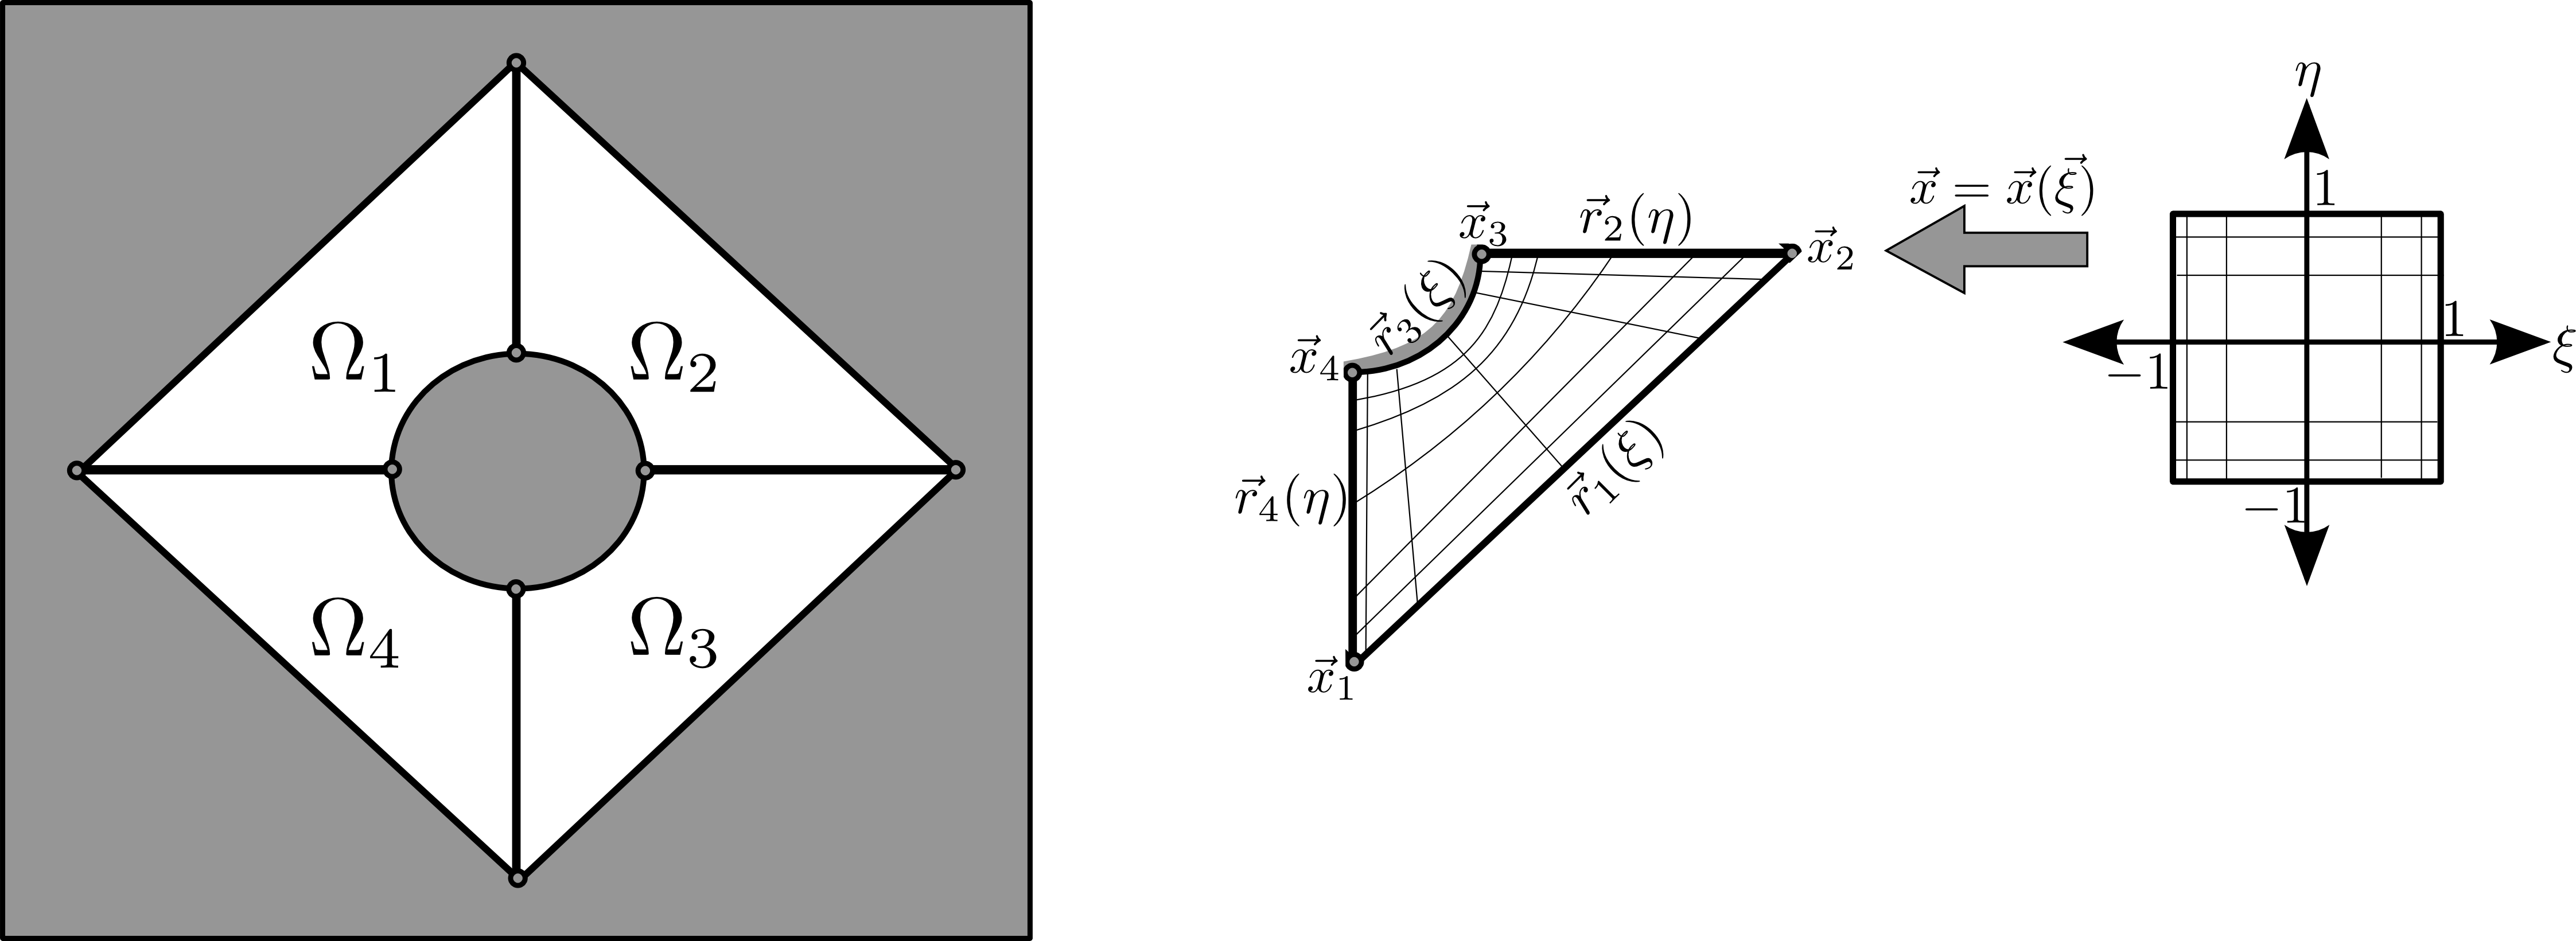
\includegraphics[width=0.9\textwidth]{../figures/geometry/meshDepiction2D-simple.png}
   \caption{A simple schematic of a spectral element mesh. This schematic shows four spectral elements, with isoparametric (curved) sides. }\label{fig:simplemesh}
\end{center}
\end{figure} 
 
 
\section{Spectral Element Methods} 
First, we discuss a taxonomy of SEMs and relate them to general Spectral Methods and Pseudo-Spectral methods in order to provide context. In general, spectral methods refer to the numerical algorithms which estimate solutions to PDEs and have error convergence rates that depend only on the smoothness of the solution. This error convergence is obtained by approximating the solution by a linear combination of basis functions. The choice in basis function is usually motivated by the application. For example, periodic systems can easily make use of Fourier basis which automatically satisfy periodic boundary conditions. Other problems in which the prescription of arbitrary boundary conditions is necessary make use of Jacobi polynomials. Historically, Chebyshev and Legendre polynomials have been used. In addition to the choice in basis function, the PDE can be approximated in the strong or the weak form. So-called ``pseudo-spectral'' methods approximate the strong form while \textit{Galerkin} methods approximate the weak form. 

Galerkin methods have typically been used for problems with complicated geometry where an unstructured mesh is necessary; these are \textit{multi-domain} methods. In these problems, the physical domain is decomposed into many ``spectral elements''. Over each element, the solution is approximated by a suitable polynomial basis. The global solution is constructed by piecewise polynomial interpolation. Galerkin methods which require continuity between spectral elements are called \textit{Continuous Galerkin Spectral Element Methods} (CGSEMs). Those which do not enforce continuity are \textit{Discontinuous Galerkin Spectral Element Methods} (DGSEMs). Historically, CGSEMs have been applied to elliptic and parabolic PDEs while DGSEMs have been applied to hyperbolic problems.  

\chapter{SEM Discretizations}
The main focus of the software is on Legendre-Galerkin Spectral Element Methods, though it is trivial to add other polynomial bases. The software can be broken into two distinct components:
\begin{enumerate}
\item SEM algorithm core
\item Geometry
\end{enumerate}
Both of these components rely on interpolants, and in this sense interpolation routines comprise the basic building block of the Spectral Element Methods. Here we start with an outline of \textit{projection}, interpolation, differentiation, and integration.

\section{Projection, Interpolation, Differentiation, and Integration}

A generic discretization is outlined for hyperbolic conservation laws to motivate the necessary modular components of the software for DGSEMs. Similarly, a generic elliptic or parabolic PDE is discretized to motivate the modular components of the software for CGSEMs. This illustrates how the two distinct components can be used together to solve PDEs in complicated geometry. Additionally, this exposition will outline the necessary attributes of data-structures that will be used in an object-oriented approach.

\section{DGSEM}\label{sec:DGSEMtheory}
A conservation law can be written in the form
  \begin{equation}
 \vec{s}_t + \nabla \cdot \vec{f} + \vec{q} = 0, \label{eq:ConservationForm}
 \end{equation}
 where $\vec{s}$ is a vector of \textit{prognostic} variables, $\vec{f}$ is a vector of \textit{conservative flux vectors} and $\vec{q}$ is a vector of \textit{non-conservative source terms}.
 
The DGSEM discretizes \eqref{eq:ConservationForm} in its weak form. To obtain the weak form, \eqref{eq:ConservationForm} is weighted with a test function and integrated over the physical domain, call it $\Omega$. To approximate the integrals in the weak form, the domain is first divided into non-overlapping elements  ($\Omega^\kappa$) . Integration is performed over each element and the solution and test function are permitted to be piecewise discontinuous across elements. These assumptions lead to the statement
  \begin{equation}
  \int_{\Omega^\kappa} (\vec{s}_t + \vec{q} )\phi \hspace{1mm} d\Omega^\kappa  - \int_{\Omega^\kappa} \vec{f} \cdot \nabla \phi \hspace{1mm} d\Omega^\kappa + \oint_{\partial \Omega^\kappa} \phi \vec{f}\cdot \hat{n} \hspace{1mm} d A^\kappa = 0, \hspace{3mm} \forall \phi \in \mathbb{C}_0(\Omega_\kappa), \hspace{2mm} \kappa=1,2,...,K \label{eq:weakForm}
  \end{equation}
where $\mathbb{C}_0(\Omega^\kappa)$ is the space of functions that are continuous over $\Omega^\kappa$.

Equation \eqref{eq:weakForm} assumes that the integration over each element is independent; this \textit{compactness} results from allowing piecewise discontinuous solutions. The third term in \eqref{eq:weakForm} is the integral of the conservative flux over the element boundary. This is the only term that involves communication with other elements. For hyperbolic problems, this communication is only between \textit{neighboring elements} which share a common node (1-D), edge (2-D), or face (3-D).

  The formulation presented in \eqref{eq:weakForm} only requires that we know the geometry of each element and the connectivity of a collection of elements. This allows for the use of either structured or unstructured mesh frameworks. Additionally, the elements which comprise the mesh can have curvilinear geometry. Define the mapping from physical space $\vec{x}$ to computational space $\vec{\xi}$ using
  \begin{equation}
  \vec{x} = \vec{x}(\vec{\xi}).\label{eq:mapping}
  \end{equation}
  Section \ref{sec:GeometryTheory} provides the details on the metric terms that are introduced along with the form of the divergence, gradient, and curl under such a mapping. For simplicity, the computational domain is formed from tensor products of intervals $[-1, 1]$ in each coordinate direction. This criteria restricts the elements to be logically segments (1-D), quadrilaterals (2-D), or hexahedrons (3-D). Under the mapping \eqref{eq:mapping}, the weak form \eqref{eq:weakForm} becomes
  \begin{equation}
  \int_{\Omega^\xi} (\tilde{s}^\kappa_t + \tilde{q}^\kappa) \phi \hspace{1mm} d\Omega^\xi  - \int_{\Omega^\xi} \tilde{f}^\kappa \cdot \nabla_{\vec{\xi}} \phi  \hspace{1mm} d\Omega^\xi + \oint_{\partial \Omega^\xi} \phi \tilde{f}^{\kappa,*}  \cdot \hat{n}^\xi \hspace{1mm} d A^\xi = 0, \hspace{2mm} \forall \phi \in \mathbb{C}^0(\Omega^\xi) \label{eq:mappedWeakForm}
  \end{equation}
  where $\tilde{s} = J^\kappa\vec{s}$, $\tilde{q} = J^\kappa\vec{q}$, $\tilde{f} = ( J^\kappa \vec{a}^{\kappa,i} \cdot \vec{f} ) \hat{a}^{\kappa,i}$, $J^{\kappa}$ is the Jacobian of the transformation over the $\kappa^{th}$ element, and $\vec{a}^{\kappa,i}$ are the contravariant basis vectors associated with the transformation of element $\kappa$ (the $\hat{a}$ denotes a unit vector).\\
  
 Given a conservative flux, a non-conservative source, internal element metrics, and global element connectivity, the discrete algorithm solves \eqref{eq:mappedWeakForm} by approximating the integrands with interpolants and the integrals by discrete quadratures. First, the prognostic solution, source term, conservative flux, and mapping are approximated by Lagrange interpolants of degree N.
 \begin{subequations}
    \begin{align}
    \vec{s} &\approx I^N(\vec{s}) = \sum_{i,j,k=0}^N \vec{S}_{i,j,k} l_i(\xi^1) l_j(\xi^2) l_k(\xi^3) \\
    \vec{q} &\approx I^N(\vec{q}) = \sum_{i,j,k=0}^N \vec{Q}_{i,j,k} l_i(\xi^1) l_j(\xi^2) l_k(\xi^3) \\
    \vec{f} &\approx I^N(\vec{f}) = \sum_{i,j,k=0}^N \vec{F}_{i,j,k} l_i(\xi^1) l_j(\xi^2) l_k(\xi^3) \\
    \vec{x} &\approx I^N( \vec{x} ) = \sum_{i,j,k=0}^N \vec{X}_{i,j,k} l_i(\xi^1) l_j(\xi^2) l_k(\xi^3)
    \end{align}
 \end{subequations}
An additional simplification is to approximate the product of interpolants by an interpolant of degree $N$ which incurs an additional aliasing error.
\begin{subequations}
    \begin{align}
    \tilde{s} &\approx I^N(I^N(J) I^N(\vec{s})) = \tilde{S} =  \sum_{i,j,k=0}^N (J \vec{S}_{i,j,k}) l_i(\xi^1) l_j(\xi^2) l_k(\xi^3) \\
    \tilde{q} &\approx I^N(I^N(J) I^N(\vec{q}))= \tilde{Q} = \sum_{i,j,k=0}^N (J \vec{Q})_{i,j,k} l_i(\xi^1) l_j(\xi^2) l_k(\xi^3) \\
    \tilde{f}_{(i,n)} &\approx I^N(I^N(Ja^i_{(n)})I^N(\vec{f}) ) =\tilde{F}_{(i,n)}= \sum_{i,j,k=0}^N (Ja^i_{(n)}\vec{F}_{(n)})_{i,j,k} l_i(\xi^1) l_j(\xi^2) l_k(\xi^3) 
    \end{align}
 \end{subequations}
 
Last, the space of test functions ($\mathbb{C}_0$) is approximated by the $\mathbb{P}^N$, the space of polynomials of degree $N$. Thus, the test function $\phi$ is replaced by each of the Lagrange interpolating polynomials, 
 \begin{equation}
 \phi_{m,n,p} = l_m(\xi^1) l_n(\xi^2) l_p(\xi^3)
 \end{equation}
 With this, equation \eqref{eq:mappedWeakForm} becomes
   \begin{equation}
  \int_{\Omega^\xi} (\tilde{S}^\kappa_t + \tilde{Q}^\kappa) \phi_{m,n,p}  \hspace{1mm} d\Omega^\xi  - \int_{\Omega^\xi} \tilde{F}^\kappa \cdot \nabla_{\vec{\xi}} \phi_{m,n,p}   \hspace{1mm} d\Omega^\xi + \oint_{\partial \Omega^\xi} \phi_{m,n,p}  \tilde{F}^{\kappa,*}  \cdot \hat{n}^\xi \hspace{1mm} d A^\xi = 0, \hspace{2mm} m,n,p=0,1,...,N  \label{eq:approx_mappedWeakForm}
  \end{equation}
  
The final step is to replace the integrals in \eqref{eq:approx_mappedWeakForm} with discrete quadrature. For this we use the Legendre-Gauss quadrature, which yields exact integration for each term in \eqref{eq:approx_mappedWeakForm}. Additionally, the interpolation nodes are specified as the Legendre-Gauss nodes, which simplifies the integration. The algorithm is now presented in one, two, and three dimesnions.

\subsection{Algorithm in One-Dimensions}\label{sec:DGSEM_1D}
In one-dimension, the global physical domain is partitioned into a set of line segments. The first term in \eqref{eq:approx_mappedWeakForm} becomes
\begin{equation}
\int_{\Omega^\xi} \tilde{S}^\kappa_t \phi_{m}  \hspace{1mm} d\Omega^\xi = \sum_{\alpha=0}^N\left[ \sum_{i=0}^N\left( (\tilde{S}^\kappa_{i})_tl_i(\xi_\alpha) \right)  l_m(\xi_\alpha) \omega_\alpha\right] \label{eq:discreteMass}
\end{equation}
where the $\xi_\alpha$ are the Legendre-Gauss nodes and the $\omega_m$ are the Legendre-Gauss weights. Since the interpolation nodes are equivalent to the quadrature nodes, \eqref{eq:discreteMass} is greatly simplified by the use of the Kronecker-delta property of Lagrange interpolating polynomials,
\begin{equation}
l_i(\xi_m) = \delta_{i,m}.
\end{equation}
This yields \eqref{eq:discreteMass} as
\begin{equation}
\int_{\Omega^\xi} \tilde{S}^\kappa_t \phi_{\alpha}  \hspace{1mm} d\Omega^\xi = (\tilde{S}^\kappa_{\alpha})_t \omega_\alpha.
\end{equation}
Similarly,
\begin{equation}
\int_{\Omega^\xi} \tilde{Q}^\kappa \phi_{\alpha}  \hspace{1mm} d\Omega^\xi = \tilde{Q}^\kappa_{\alpha} \omega_\alpha.
\end{equation}
The third term in \eqref{eq:approx_mappedWeakForm} becomes
\begin{equation}
\int_{\Omega^\xi} \tilde{F}^\kappa \cdot \nabla_{\vec{\xi}} \phi_{m}   \hspace{1mm} d\Omega^\xi = \sum_{i=0}^N  \tilde{F}^\kappa_i l'_m(\xi_i) \omega_i.
\end{equation}
Lastly, the boundary flux becomes
\begin{equation}
\oint_{\partial \Omega^\xi} \phi_{\alpha}  \tilde{F}^{\kappa,*}  \cdot \hat{n}^\xi \hspace{1mm} d A^\xi = \tilde{F}^{\kappa,*}(1)l_\alpha(1) - \tilde{F}^{\kappa,*}(-1)l_\alpha(-1). 
\end{equation}
Thus, the spatially discretized system can be written
\begin{equation}
 \left( J_{m} \vec{S}_{m} \right)_t =  -\left[\sum_{i=0}^{N}\hat{D}_{m,i} \tilde{F}_{i}   + \left( \frac{ l_m(1)}{w_m} \tilde{F}^{*}(1) - \frac{ l_m(-1)}{w_m} \tilde{F}^{*}(-1) \right) \right] + J_{m}\vec{Q}_{m}; \hspace{5mm} m=0,1,...,N, \label{eq:discrete1d_system} 
\end{equation}
where
\begin{equation}
 \hat{D}_{m,i} = -\frac{l'_m(\xi_i)w_i}{w^{\xi^1}_m}
\end{equation}
is the DG-Derivative matrix. 

Up to this point, the treatment of the boundary flux has been relatively vague. In practice, the boundary flux is calculated using an approximate Riemman solver. This uses the solution state from the neighboring elements to approximate the flux across the shared boundary. The specification of the Riemman solver depends on the PDE system. Because of this, a discussion of the boundary flux is delayed until specific PDE systems are discussed.


\subsection{Algorithm in Two-Dimensions}\label{sec:DGSEM_2D}

 \begin{equation}
 \begin{split}
 \left( J_{m,n} \vec{S}_{m,n} \right)_t =  &-\left[\sum_{i=0}^{N}\hat{D}^{(\xi^1)}_{m,i} \tilde{F}^{(\xi^1)}_{i,n}   + \left( \frac{ l_m(1)}{w^{(\xi^1)}_m} \tilde{F}^{*}(1,\xi^2_n) - \frac{ l_m(-1)}{w^{(\xi^1)}_m} \tilde{F}^{*}(-1,\xi^2_n) \right) \cdot \hat{\xi^1} \right] \\
  &-\left[ \sum_{j=0}^{N}\hat{D}^{(\xi^2)}_{n,j} \tilde{F}^{(\xi^2)}_{m,j}  + \left( \frac{l_n(1)}{w^{(\xi^2)}_n} \tilde{F}^{*}(\xi^1_m,1)  -  \frac{l_n(-1)}{w^{(\xi^2)}_n} \tilde{F}^{*}(\xi^1_m,-1) \right)\cdot \hat{\xi^2}  \right] \\ 
 &+ J_{m,n}\vec{Q}_{m,n}; \hspace{5mm} m,n=0,1,...,N
\end{split} \label{eq:discrete2d_system} 
 \end{equation}

 Computing the divergence of the conservative flux in this framework can be viewed as calculating a sequence of derivatives in each computational direction. Two steps are required to compute the derivative in each direction. The first is an internal matrix-vector multiply, and the second is computing the weighted Riemann fluxes at the element boundaries. The latter is the only step which requires element-to-element communication.
 
 \subsection{Algorithm in Three-Dimensions}
 \begin{equation}
 \begin{split}
 \left( J_{m,n,p} \vec{S}_{m,n,p} \right)_t =  &-\left[\sum_{i=0}^{N}\hat{D}^{(\xi^1)}_{m,i} \tilde{F}^{(\xi^1)}_{i,n,p}   + \left( \frac{ l_m(1)}{w^{(\xi^1)}_m} \tilde{F}^{*}(1,\xi^2_n,\xi^3_p) - \frac{ l_m(-1)}{w^{(\xi^1)}_m} \tilde{F}^{*}(-1,\xi^2_n,xi^3_p) \right) \cdot \hat{\xi^1} \right] \\
 &-\left[ \sum_{j=0}^{N}\hat{D}^{(\xi^2)}_{n,j} \tilde{F}^{(\xi^2)}_{m,j,p}  + \left( \frac{l_n(1)}{w^{(\xi^2)}_n} \tilde{F}^{*}(\xi^1_m,1,\xi^3_p)  -  \frac{l_n(-1)}{w^{(\xi^2)}_n} \tilde{F}^{*}(\xi^1_m,-1,\xi^3_p) \right)\cdot \hat{\xi^2}  \right] \\
 &-\left[ \sum_{k=0}^{N}\hat{D}^{(\xi^3)}_{m,n,k} \tilde{F}^{(\xi^2)}_{m,n,k}  + \left( \frac{l_p(1)}{w^{(\xi^3)}_p} \tilde{F}^{*}(\xi^1_m,\xi^2_n,1)  -  \frac{l_p(-1)}{w^{(\xi^3)}_p} \tilde{F}^{*}(\xi^1_m,-\xi^2_n,-1) \right)\cdot \hat{\xi^3}  \right] \\ 
 &+ J_{m,n,p}\vec{Q}_{m,n,p}; \hspace{5mm} m,n,p=0,1,...,N
\end{split} \label{eq:discrete3d_system} 
 \end{equation}
 
\section{CGSEM}
\section{Geometry}\label{sec:GeometryTheory}

\section{Code Organization}
Two classes of SEMs have been presented. Both require the use of Lagrange interpolating polynomials and Legendre Gauss or Gauss-Lobatto quadrature. This necessitates the development of low level support modules which provide a data structure and routines for interpolation and differentation. Auxiliary routines are provided separately to provide the Legendre Gauss or Gauss-Lobatto nodes and weights. To calculate the solution tendency, the solution at the quadrature nodes and at the boundaries is needed. Additionally, the quadrature weights and (some form of) the derivative matrix are needed. This motivates the development of two data structures. The first stores the ``book-keeping'' information such as the interpolant, derivative matrix, and the quadrature weights. The second stores the solution, flux, and tendency (for the DGSEM). Lastly, it was seen that a data structure is needed for handling the SE mesh information such as the element, edge, and node connectivity and internal geometry of each element. Together, these modules can be used to develop ``high-end'' solvers PDE systems. Under each class of modules, a single module is developed for one, two, and three dimensions.


\chapter{Modules}
\section{Interpolation, Differentiation, and Integration}


\section{Geometry}

\section{Solution Storage}

\section{Template DGSEM}

\section{Template CGSEM}

\section{Filters}
Models are just that, they're models. We cannot currently hope to explicitly and accurately represent all of the spatial and temporal scales for a problem. Instead, models focus in on the spatial and temporal scales that are important and an informed decision is made to deal with the interactions with smaller scales. In the prototypical problem of shock formation (a la Burger's equation), small scales are forced into existence from the large scale. This nonlinear transfer of energy to small scales, called the ``forward cascade'', poses challenges for numerical models that can become unstable when too much energy is forced into the smallest resolvable scale. The comic shown in Fig. \ref{fig:shockFormation} shows what happens when you don't remove that energy from the grid scale (the red line). The blue line shows the same shock formation occurring, except that the numerical algorithm now includes a "filter" that turns on when too much energy appears in the grid-scale and violates the principles of the forward cascade (it is called ``adaptive'' because of its conditional action). The filter effectively removes the oscillations, so-called ``grid-scale noise'', and removes enough energy to maintain stable numerical integration. The filter used in generating the stable solution in Fig. \ref{fig:shockFormation} is a "Roll-off" filter, meaning that it damps marginally resolved modes much stronger than the well resolved modes. This Adaptive Roll-off Filter (ARF) is a parameterization for shock formation. Motivated by the need for maintaining numerical stability in a justifiable manner, a set of filters are provided with the SELF as one option towards meeting this goal. In this section, the theory behind using filters is presented for 1-D. The advantage that polynomial filtering has over other parameterizations (e.g. Laplacian diffusion), is that the additional error incurred by such a filter is quantifiable.

\begin{figure}
\begin{center}
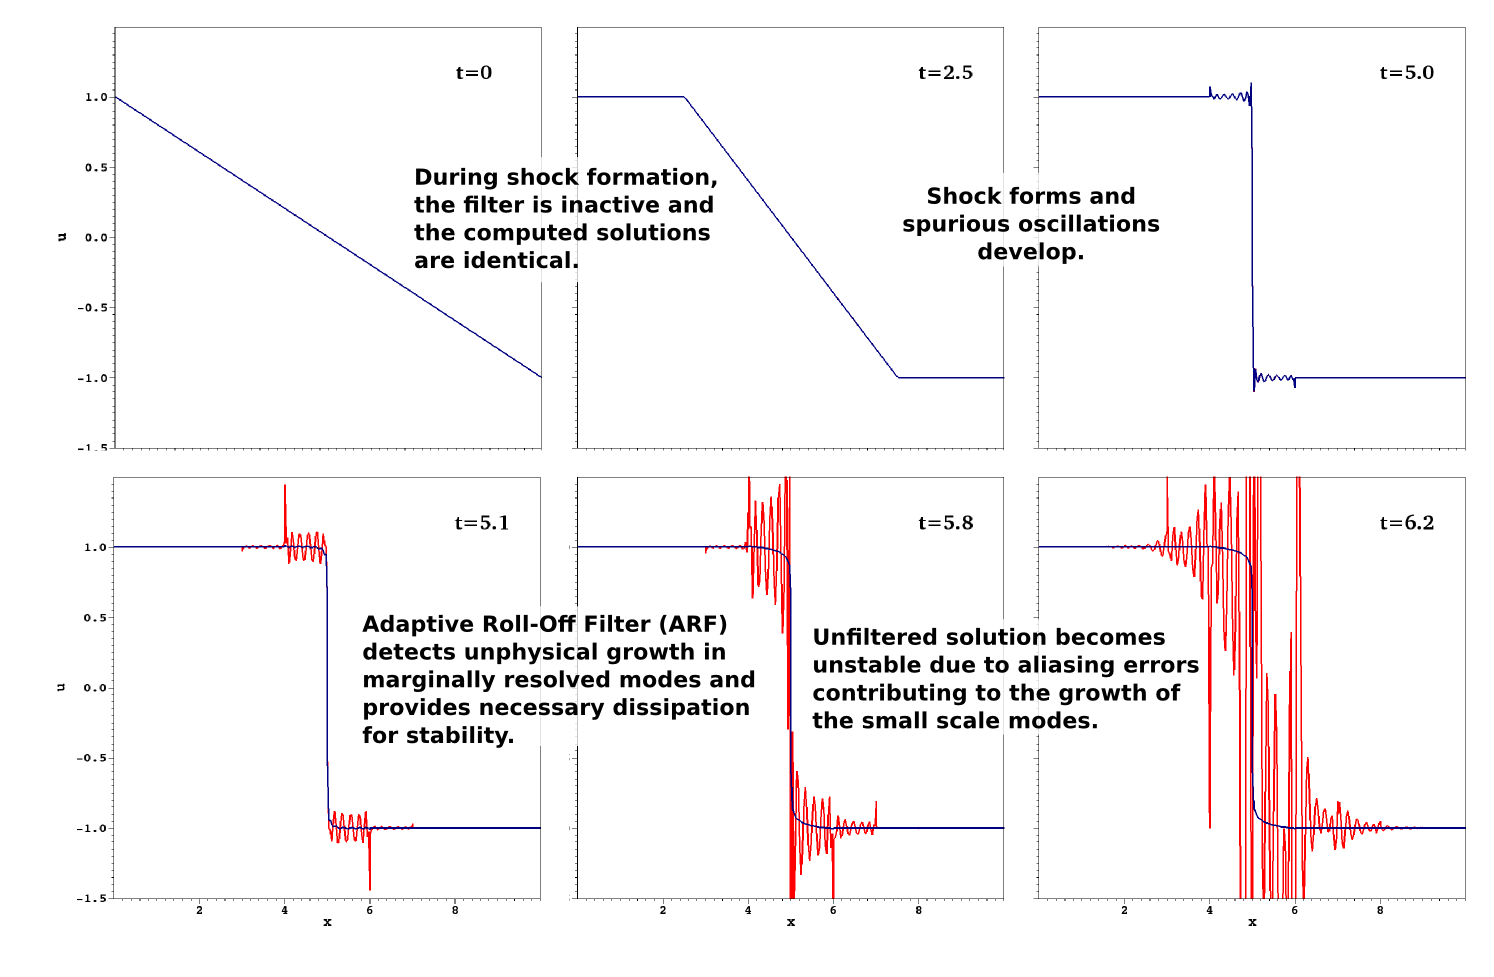
\includegraphics[width=0.9\textwidth]{../figures/filters/burger1d-ARF15h10l/Comic-FilterDemo.png}
\caption{}\label{fig:shockFormation}
\end{center}
\end{figure}

In the ``standard'' nodal discretization of conservation laws presented in Eqns. \eqref{eq:discrete1d_system} \eqref{eq:discrete2d_system} and \eqref{eq:discrete3d_system}, additional aliasing errors can arise in approximating the flux by a polynomial of the same degree as the solution. This is always the case when the flux depends nonlinearly on the solution. The introduction of aliasing errors directly implies inexactness of the discrete integration and hence stability of the spatial discretization does not follow. However, the quadrature order can be increased in order to remove these aliasing errors which can then restore stability (provided the continuous problem is well posed). This approach is known as \textit{over-integration}. In theory, over-integration would involve interpolation of the solution onto a higher order mesh, integration of the flux, and mapping back to the lower order mesh. In practice, this process can be done more efficiently by \textit{polynomial de-aliasing} \citep{Gassner2013,Flad2016}. In the de-aliasing framework, over-integration is achieved by applying a \textit{modal-cutoff filter} to the solution variable that effectively projects the solution to a polynomial of low-enough degree so that the integration of the flux is exact.

As an example, suppose we are interested in solving Burger's equation in 1-D, as in Fig. \ref{fig:shockFormation}, 
\begin{subequations}
\begin{align}
 u_t + \left(\frac{u^2}{2}\right)_x &= 0 \\
 u(0,t) &= 1 \\
 u(10,t) &= -1 \\
 u(x,0) &= -\frac{2x}{10} + 1
\end{align}
\end{subequations}\label{eq:burgersEx}
If $u$ is approximated by a polynomial of degree $N$, then the integrand in the discretized system \eqref{eq:discrete1d_system} for the flux integral is of degree $3N$. Gauss quadrature of order $M$ is exact for integrands of degree $2M+1$, so 
\begin{equation}
3N = 2M+1 \label{eq:exactness}
\end{equation}
guarantees exactness of the discrete integration and stability of the spatial discretization. In practice, the discretization of \eqref{eq:burgersEx} would be performed at degree $M$, and at every iteration the solution would be projected onto a polynomial of degree $N$ that satisfies the exactness criteria \eqref{eq:exactness}.

\subsection{How to de-alias}
Recall that the approximate solution can be expressed in \textit{nodal} or \textit{modal} form :
\begin{equation}
u \approx I_M[u] = \sum_{i=0}^M U_i l_i(\xi) = \sum_{j=0}^{M} \hat{U}_j L_j(\xi) \label{eq:nodalAndModal}
\end{equation}
where the $U_i$ are the nodal values of the interpolant, $l_i$ are the Lagrange interpolating polynomials and $\hat{U}_j$ are the modal coefficients of the Legendre basis functions $L_j$. Other polynomial bases can be used, but here our attention is restricted to Legendre polynomials. Gauss quadrature of order $M$ guarantees discrete orthogonality between the Legendre polynomials up to degree $M$. Because of this, weighting \eqref{eq:nodalAndModal} with each Legendre polynomial and performing discrete integration provides a formula for each of the modal coefficients,
\begin{equation}
\hat{U}_m = \sum_{k=0}^M U_k \frac{L_m(\xi_k) \sigma_k}{||L_m||^2_M} \label{eq:ModalCoeffs}.
\end{equation}
Eq. \eqref{eq:ModalCoeffs} can be conveniently be written in matrix form
\begin{equation}
\hat{U} = T \vec{U}
\end{equation}
where $\hat{U}$ is a vector of the modal coefficients, $\vec{U}$ is a vector of the nodal values, and $T_{m,k} = \frac{L_m(\xi_k) \sigma_k}{||L_m||^2_M} $ is the nodal-to-modal transformation matrix. The inverse of $T$ transforms from the modal space to the nodal space and is easily obtained by evaluating the Legendre polynomials at the interpolation nodes :
\begin{equation}
T^{-1}_{m,k} = L_{k}(\xi_m) \label{eq:ModalToNodal}
\end{equation}
Filtering is done by transforming the nodal values to the modal coefficients, modifying the modal coefficients, and applying the inverse to map the ``filtered'' interpolant back to the nodal values.
\begin{enumerate}
\item Obtain the modal coefficients : $\hat{U} = T \vec{U}$ 
\item Apply a filter on the modal coefficents : $\tilde{U} = P\hat{U} = PT\vec{U}$
\item Map from the filtered modal coefficients to the nodal coefficients : $\vec{U}_{f} = (T^{-1}PT)\vec{U}$
\end{enumerate}
When de-aliasing, the modal coefficients associated with Legendre polynomials higher than degree $N$ are set to zero identically, so that the interpolant is effectively projected onto a lower order polynomial. The modal filter matrix that does this is a diagonal matrix with
\begin{equation}
P_{i,i} = 
\begin{cases}
     1, & \text{if } i \leq N \\
     0, & \text{otherwise}
\end{cases}\label{eq:cutoff}
\end{equation}
The matrix $T^{-1}PT$ with $P$ given by \eqref{eq:cutoff} is called a \textit{modal-cutoff filter}.

\chapter{Software Validation}
\section{Lagrange Interpolation}

\subsection{ Guassian Bump in 1-D }
 This example tests the functionality of the following modules :
 \begin{enumerate}
 \item Legendre.f90
 \item Lagrange\_1D\_Class.f90
 \end{enumerate}
 By interpolating through the Legendre-Gauss nodes, the error in the interpolating function should decay spectrally with increasing interpolating polynomial degree \citep{Kopriva2009}. The interpolant can be expressed as the sum of the actual function and an interpolation error, 
\begin{equation}
I_N[ f(s) ] = f(s)  + \epsilon(N),
\end{equation} 
where $I_N[ f(s) ]$ denotes the interpolation of $f(s)$ by a degree $N$. When the evaluation nodes are the Legendre Gauss nodes, $\epsilon(N)$ is a spectrally small error; it's rate of decay with $N$ depends on the smoothness of $f$. Additionally, the derivative of the interpolant approximates the derivative of the function. 
  \begin{equation}
  \frac{d}{ds}[ I_N(f) ] = \frac{df}{ds} + \delta(N)
  \end{equation}
 where $\delta(N)$ is also a spectrally small error. For the interpolation of smooth functions, the error decays exponentially with $N$.s
 
 A test program (\texttt{$\sim$/src/interp/Testing/TestLagrangeInterpolation\_1D.f90}) has been written to interpolate the function 
 \begin{equation}
 f(s) = e^{-s^2}
 \end{equation}
 and estimate the $\mathbb{L}_2$ error of the interpolation and differentiation. Differentiation is carried out by building the derivative matrix (\texttt{S/R CalculateDerivativeMatrix}) and performing a matrix vector multiply (\texttt{MATMUL}). The $\mathbb{L}_2$ error is estimated using Legendre-Gauss quadrature with 50 evaluation nodes, ie, 
 \begin{equation}
 || f - I_N[f] ||_{\mathbb{L}_2} = \sum_{k=0}^K \left( f(s_k) - I_N[f(s_k)] \right)^2 \sigma_k
 \end{equation}
 where $s_k$ and $\sigma_k$ are the degree $K$ Legendre Gauss quadrature nodes quadrature weights respectively. 
 



Figures \ref{fig:GaussianFunction} and \ref{fig:GaussianDerivative} show the interpolants and the interpolant derivatives respectively for polynomial degrees $N=2$ through $N=7$. Qualtitatively, these plots illustrate the convergence of the interpolants to the exact function and derivative. Figure \ref{fig:Errors} shows the $\mathbb{L}_2$ error norm in approximating the function and the derivative for polynomial degrees 2 through 17. Both errors exhibit exponential convergence, in agreement with the theoretical error bounds. Notice that the error in approximating the function is always smaller than in approximating its derivatine (for each polynomial degree). This indicates that approximating the derivative by taking the derivative of the interpolant incurs an additional error; the derivative of the interpolant is not always equal to the interpolant of the derivative.

Given that the function being interpolated is complete (we can take as many derivatives as we like), the theoretical error decay is exponential. This is in agreement with the error trend observed numerically, providing evidence that the interpolation and differentiation routines at the Legendre Gauss nodes are working.

  


\pagebreak
\bibliography{refs}
\bibliographystyle{plainnat}

\end{document}


\begin{figure}
\begin{center}

   \begin{tikzpicture}
      \begin{axis}[
        width=0.65\textwidth,
        height=0.45\textwidth,
        axis line style=very thick, 
        title style = {font=\sansmath\sffamily},
        xmin=-1,
        xmax=1,
        ymin=0,
        ymax=1.2,
        enlargelimits=false,
        legend style={at={(1.01,0.5)},anchor=west} ,       
        xlabel={$s$},
        ylabel={$I_N[f(s)]$},
        title={}
        ]
       \addplot[
          color=green,
          mark=none,
          very thick
          ]      
          table{data/interp/lag1d_gaussianTest/f.00002.curve};
       \addplot[
          color=orange,
          mark=none,
          very thick
          ]      
          table{data/interp/lag1d_gaussianTest/f.00003.curve};
          \addplot[
          color=violet,
          mark=none,
          very thick
          ]      
          table{data/interp/lag1d_gaussianTest/f.00004.curve};
          \addplot[
          color=blue,
          mark=none,
          very thick
          ]      
          table{data/interp/lag1d_gaussianTest/f.00005.curve};
          \addplot[
          color=black,
          mark=none,
          very thick
          ]      
          table{data/interp/lag1d_gaussianTest/f.00006.curve};
       \legend{$N=2$,$N=3$,$N=4$,$N=5$,$N=6$}
      \end{axis}
   \end{tikzpicture}
   \caption{ The interpolants are shown for polynomial degrees of $N=2$ through $N=6$. For presentational purposes, the interpolants are mapped to a uniform grid with 50 points.  }\label{fig:GaussianFunction}
\end{center}
\end{figure}  

\begin{figure}
\begin{center}

   \begin{tikzpicture}
      \begin{axis}[
        width=0.65\textwidth,
        height=0.45\textwidth,
        axis line style=very thick, 
        title style = {font=\sansmath\sffamily},
        xmin=-1,
        xmax=1,
        ymin=-2,
        ymax=2,
        enlargelimits=false,
        legend style={at={(1.01,0.5)},anchor=west} ,     
        xlabel={$s$},
        ylabel={$\frac{d}{ds}(I_N[f(s)])$},
        title={}
        ]
       \addplot[
          color=green,
          mark=none,
          very thick
          ]      
          table{data/interp/lag1d_gaussianTest/dfds.00002.curve};
       \addplot[
          color=orange,
          mark=none,
          very thick
          ]      
          table{data/interp/lag1d_gaussianTest/dfds.00003.curve};
          \addplot[
          color=violet,
          mark=none,
          very thick
          ]      
          table{data/interp/lag1d_gaussianTest/dfds.00004.curve};
          \addplot[
          color=blue,
          mark=none,
          very thick
          ]      
          table{data/interp/lag1d_gaussianTest/dfds.00005.curve};
          \addplot[
          color=black,
          mark=none,
          very thick
          ]      
          table{data/interp/lag1d_gaussianTest/dfds.00006.curve};
       \legend{$N=2$,$N=3$,$N=4$,$N=5$,$N=6$}
      \end{axis}
   \end{tikzpicture}
   \caption{ The derivatives of the interpolants are shown for polynomial degrees of $N=2$ through $N=6$. For presentational purposes, the derivatives are mapped to a uniform grid with 50 points using the \texttt{CoarseToFine} subroutine. }\label{fig:GaussianDerivative}
\end{center}
\end{figure} 

\begin{figure}[t!]
\begin{center}

   \begin{tikzpicture}
      \begin{axis}[
        width=0.65\textwidth,
        height=0.45\textwidth,
        axis line style=very thick, 
        title style = {font=\sansmath\sffamily},
        xmin=1,
        xmax=18,
        ymin=-23,
        ymax=0,
        enlargelimits=false,
        legend style={at={(0.98,0.98)},anchor=north east} ,      
        xlabel={N},
        ylabel={$\log_{10}$($\mathbb{L}_2$-Error)},
        title={}
        ]
       \addplot[
          color=black,
          mark=o,
          very thick
          ]      
          table{data/interp/lag1d_gaussianTest/Lagrange1D_Test_L2Errf.curve};
       \addplot[
          color=black,
          mark=x,
          very thick
          ]      
          table{data/interp/lag1d_gaussianTest/Lagrange1D_Test_L2Errdfds.curve};
       \legend{$f$, $\frac{df}{ds}$}
      \end{axis}
   \end{tikzpicture}
   \caption{ A semi-log plot of the $\mathbb{L}_2$ Error norm in approximating a gaussian function and its derivative are shown as a function of the approximating polynomial degree. The error decay is shown in this case to be exponential. }\label{fig:Errors}
\end{center}
\end{figure}